\chapter{Desenvolvimento do Projeto}

Neste capítulo é abordado tudo o que foi necessário para chegar em um projeto viável, como tecnologias utilizadas, arquitetura do sistema, viabilidade financeira, critérios necessários para segurança da aplicação, casos de uso e regrás de negócio como também métricas para dimensionar dificuldades, qualidade e tamanho do aplicativo.   



\section{Arquitetura do sistema}
A arquitetura foi escolhida visando a maior facilidade de armazenamento da aplicação na cloud do Heroku para que seja possível o acesso dela em lugares com os recursos básicos, como um dispositivo conectado a internet, e também para a equipe visulizar a evolução da construção da aplicação. 

O aplicativo diversaGente, como mostrado na \autoref{arquitetura-sistema}, está hospedado no Heroku onde atualmente está todo o back-end que é desenvolvido pelo framework nodeJS e pode receber requisições do banco de dados mongoDB e servidor de amazenamento de arquivos. O lado do cliente foi feito em React Native 

\begin{figure}[htb]
	\centering
	\caption{\label{fig_arq_virado}Arquitetura do sistema}
	\label{arquitetura-sistema}
	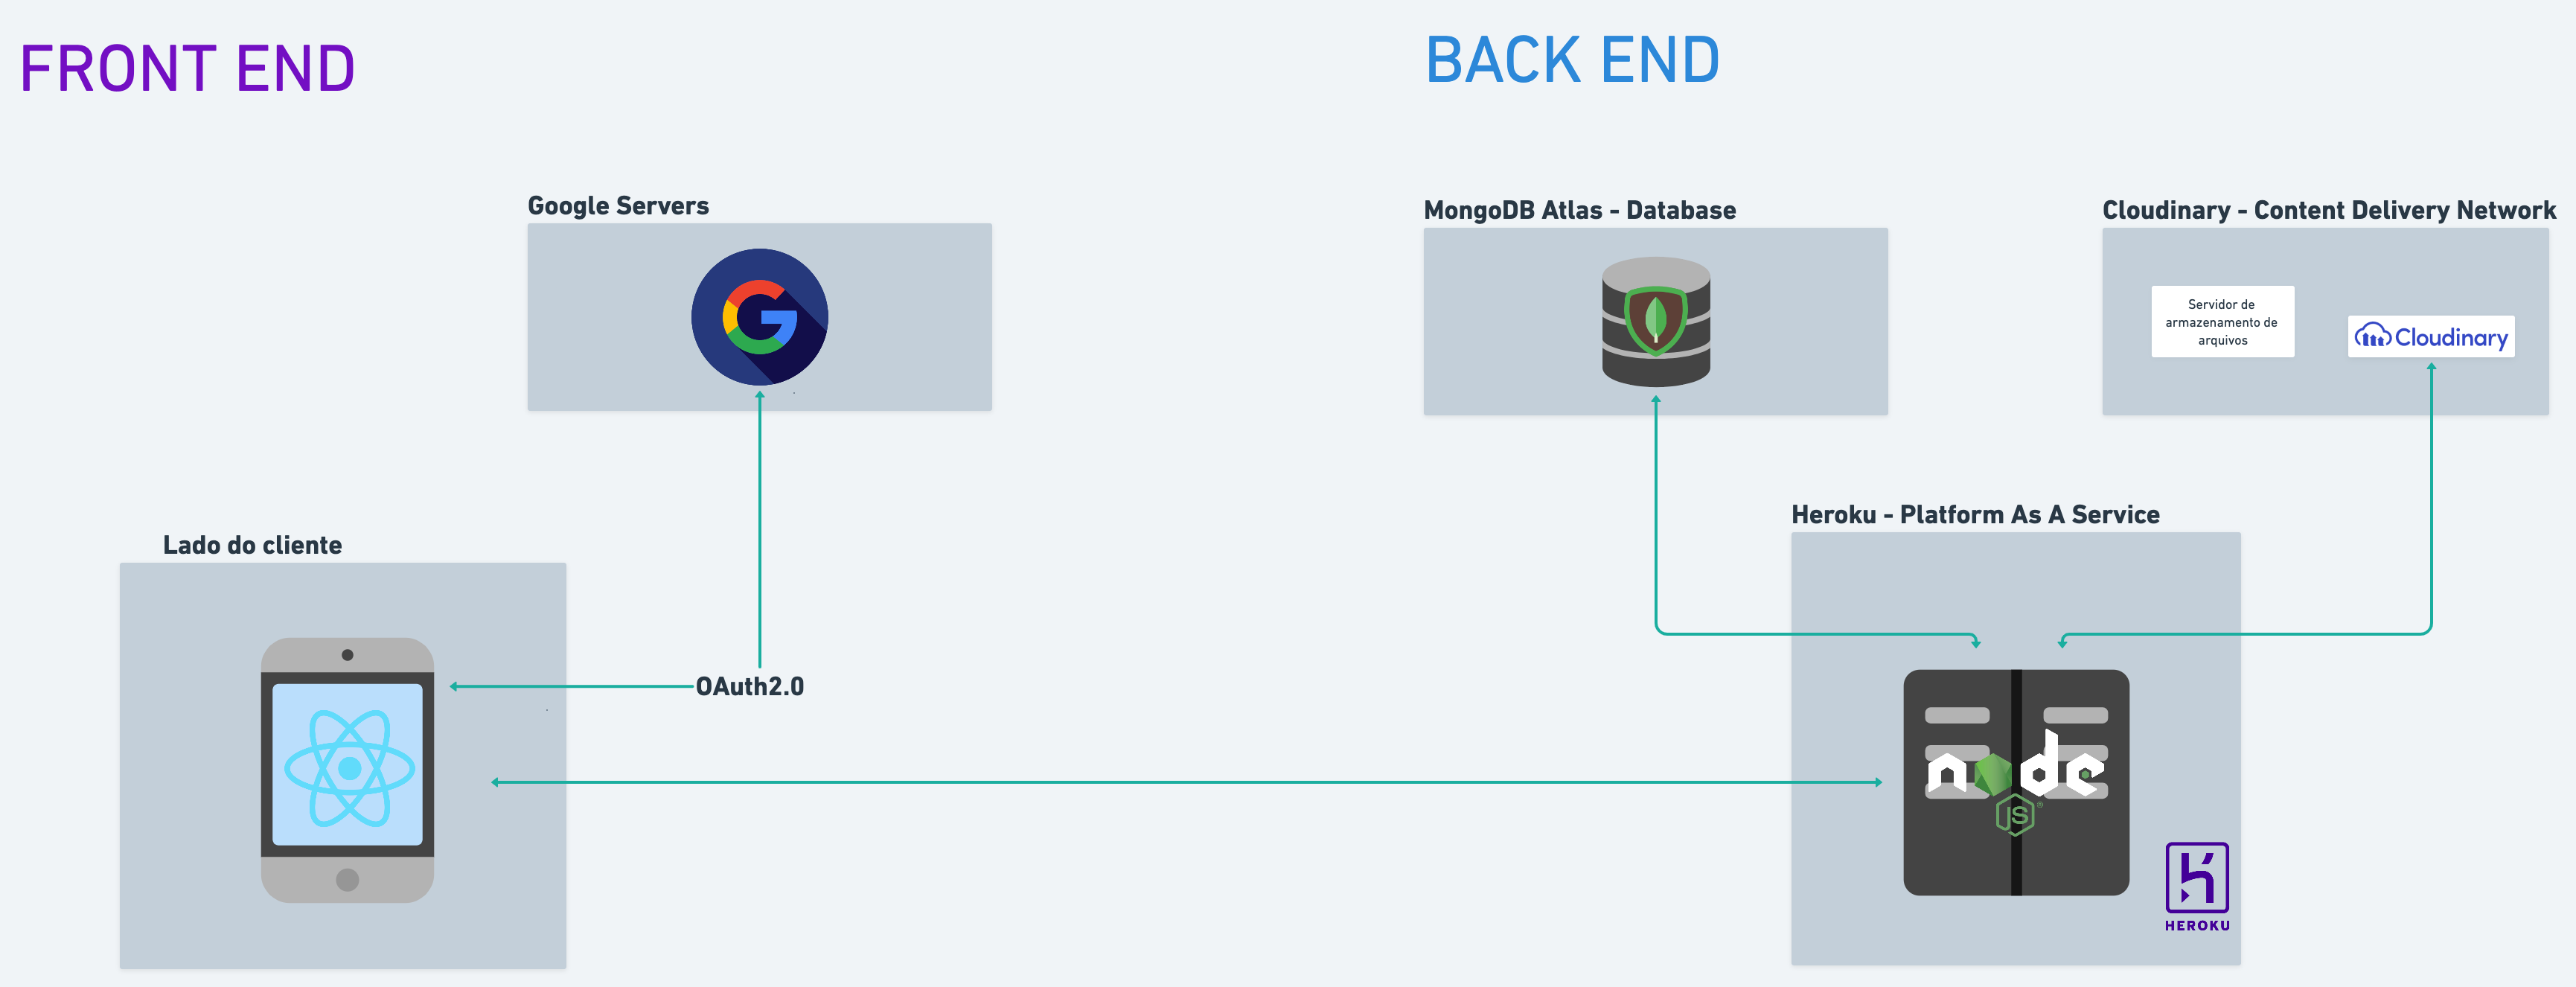
\includegraphics[width=0.9\textwidth]{anexos/poc-arquitetura.png}
	\fonte{Equipe diversaGente (2022)}
\end{figure}


\section{Tecnologias utilizadas}

Para o lado do cliente, a escolha foi o React Native com Typescript junto a ferramenta Expo para testar o app com as APIs nativas do Android que essa ferramenta disponibiliza.

Já para o lado do servidor, as ferramentas são o Node.js com Typescript e framework NestJS para a construção da API, MongoDB como banco de dados, Prisma como ORM, Cloudinary como storage e para documentação de API, a especificação OpenAPI.

Para o ambiente de desenvolvimento, a escolha foi o Docker, a fim de obter facilidade em executar o projeto independente do Sistema Operacional local.

A hospedagem é feita por meio da Play Store para o app em React Native, do Heroku para o backend em Node.js e do MongoDB Atlas para o banco de dados, e todo o versionamento feito por meio das plataformas Github e Subversion.

Para realizar a prototipação das interfaces, a opção utilizada é a ferramenta Figma e a construção de fluxos e brainstorms da equipe se dão por meio do Miro e Whimsical.

Por fim, para o gerenciamento do projeto, a escolha foi o Trello para registro de backlog e acompanhamento do status de desenvolvimento das histórias, o Discord para realização das cerimônias semanais da equipe e o WhatsApp para comunicações rápidas e mais urgentes entre o time.

\section{Escalabilidade}

O quesito ‘escalabilidade’ é muito abordado e de extrema importância atualmente, principalmente devido ao enorme fluxo de dados que corre dentre os sistemas e aplicações. A escalabilidade diz respeito a facilidade de crescimento da infraestrutura da aplicação de forma saudável, sem grandes impactos nos custos ferramentais e humanos e no desempenho da aplicação. Essa adaptabilidade pode estar relacionada com a implementação de novas funcionalidades, novas demandas de mercado, inserção em requisições legislativas e projetos de inovação, por exemplo. 

O projeto conta com ferramentas muito atuais, que já trazem consigo muito fortemente o conceito de escalabilidade, como o Heroku e o Docker, o primeiro que ganha cada vez mais espaço de mercado como uma Platform as a Service (PaaS), em que a solução permite que o desenvolvedor tenha maiores facilidades com detalhes estruturais, trazendo maior facilidade de manutenção e maior agilidade de implantação, já o segundo possibilita a criação de ambientes virtuais completos, os chamados contêineres, que podem até mesmo ter seu crescimento automatizado de acordo com a demanda de requisições, gerando novos contêineres semelhantes, por exemplo. 

Por se tratar de um modelo de aplicação com pouca concorrência em mercado, existem chances relevantes de crescimento, assim, é possível que haja a necessidade de escalada da aplicação em um futuro breve, tendo isso em consideração, as ferramentas anteriormente citadas se encaixam muito bem nessa possível necessidade futura. 



\section{Manutenibilidade e Integração Contínua}
A manutenibilidade é o que garante a qualidade do software para manutenções futuras, como corrigir erros que podem ocorrer, melhora de performance, adequar a novas práticas de mercade ou necessidade de conexão com outras aplicações. Sendo assim, utilizando as boas práticas do mercado, convenções, aplicando uma padronização e um código limpo a aplicação consegue ter uma alta manutenibilidade para quaisquer futuras adaptações.  

A integração das diversas versões de código gerado durante o desenvolvimento da aplicação foi feita através do GitHub, divididos em diversas branchs de features e para cada pessoa desenvolvedora da equipe que solicita para uma pessoa responsável pela manutenibilidade aprovar as alterações e realizar o merge com a branch principal que reflete no ambiente de produção, é possível manter os ambientes atualizados para desenvolvimento.

Para subir as alterações para o produção e conseguir fazer a visualização, foi utilizado o workflow de Continuous Integration que é gerado através do GitHub Actions



\section{Testes}

Para os testes unitários da aplicação, o Jest, um framework JavaScript para testes automatizados, e ESLint para análise estática do código.
O sistema de Log de toda aplicação Papertrail é o sistema de log escolhido para mapear o comportamento da API em Node.js.
%\pagebreak

\section{Diagrama de classes do sistema}

O diagrama de classe demonstra como que o banco de dados é modelado para a aplicação ter uma boa performance e relacionamento entre entidades. 

No diagrama de classe, \autoref{diagrama-classe}, a aplicação diversaGente, a classe User é a principal e representa o usuário que está atrelado a grande parte das outras classes, já que o objetivo principal é ser um fórum para postagem e compartilhamento de dados. 

\pagebreak

\begin{figure}[htb]
	\centering
	\caption{\label{fig_arq_virado}Diagrama de classes do sistema}
	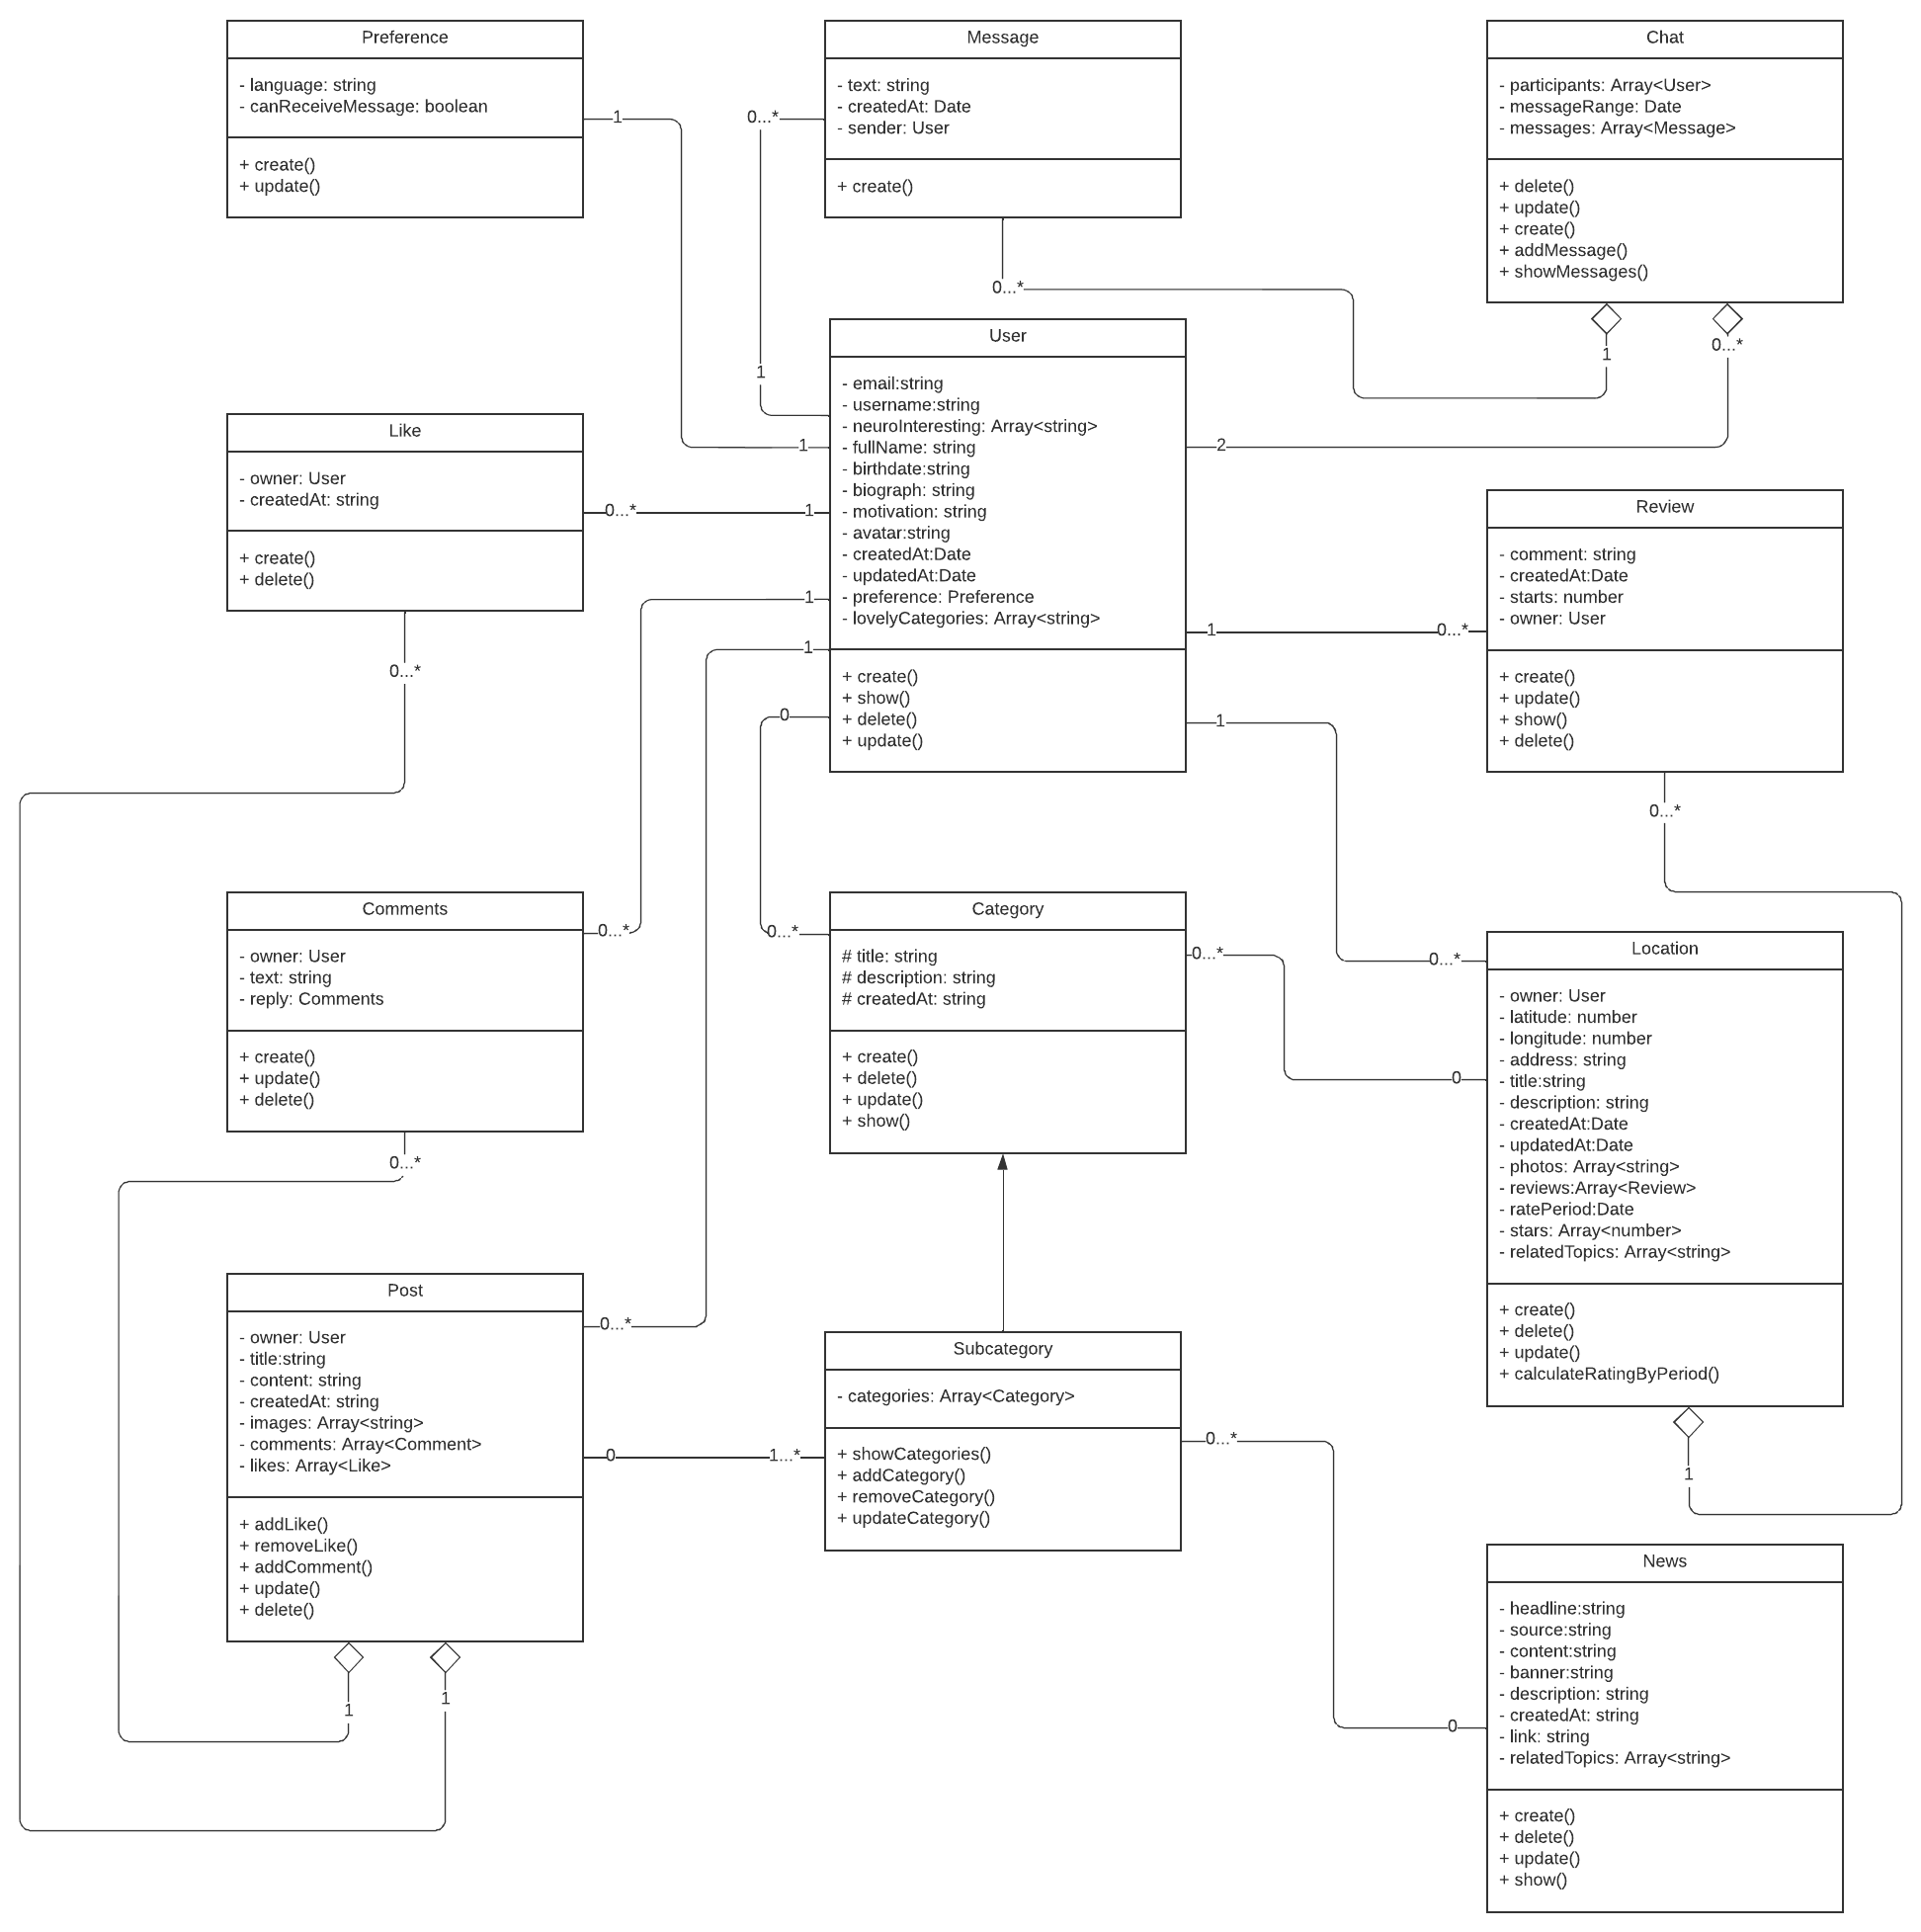
\includegraphics[width=0.90\textwidth]{anexos/diversaGente_-_Classe_UML_1.png}
	\label{diagrama-classe}
	\fonte{Equipe diversaGente (2022)}
\end{figure}
\begin{figure}[htb]
	\centering
	\caption{\label{fig_arq_virado}Diagrama de classes do sistema}
	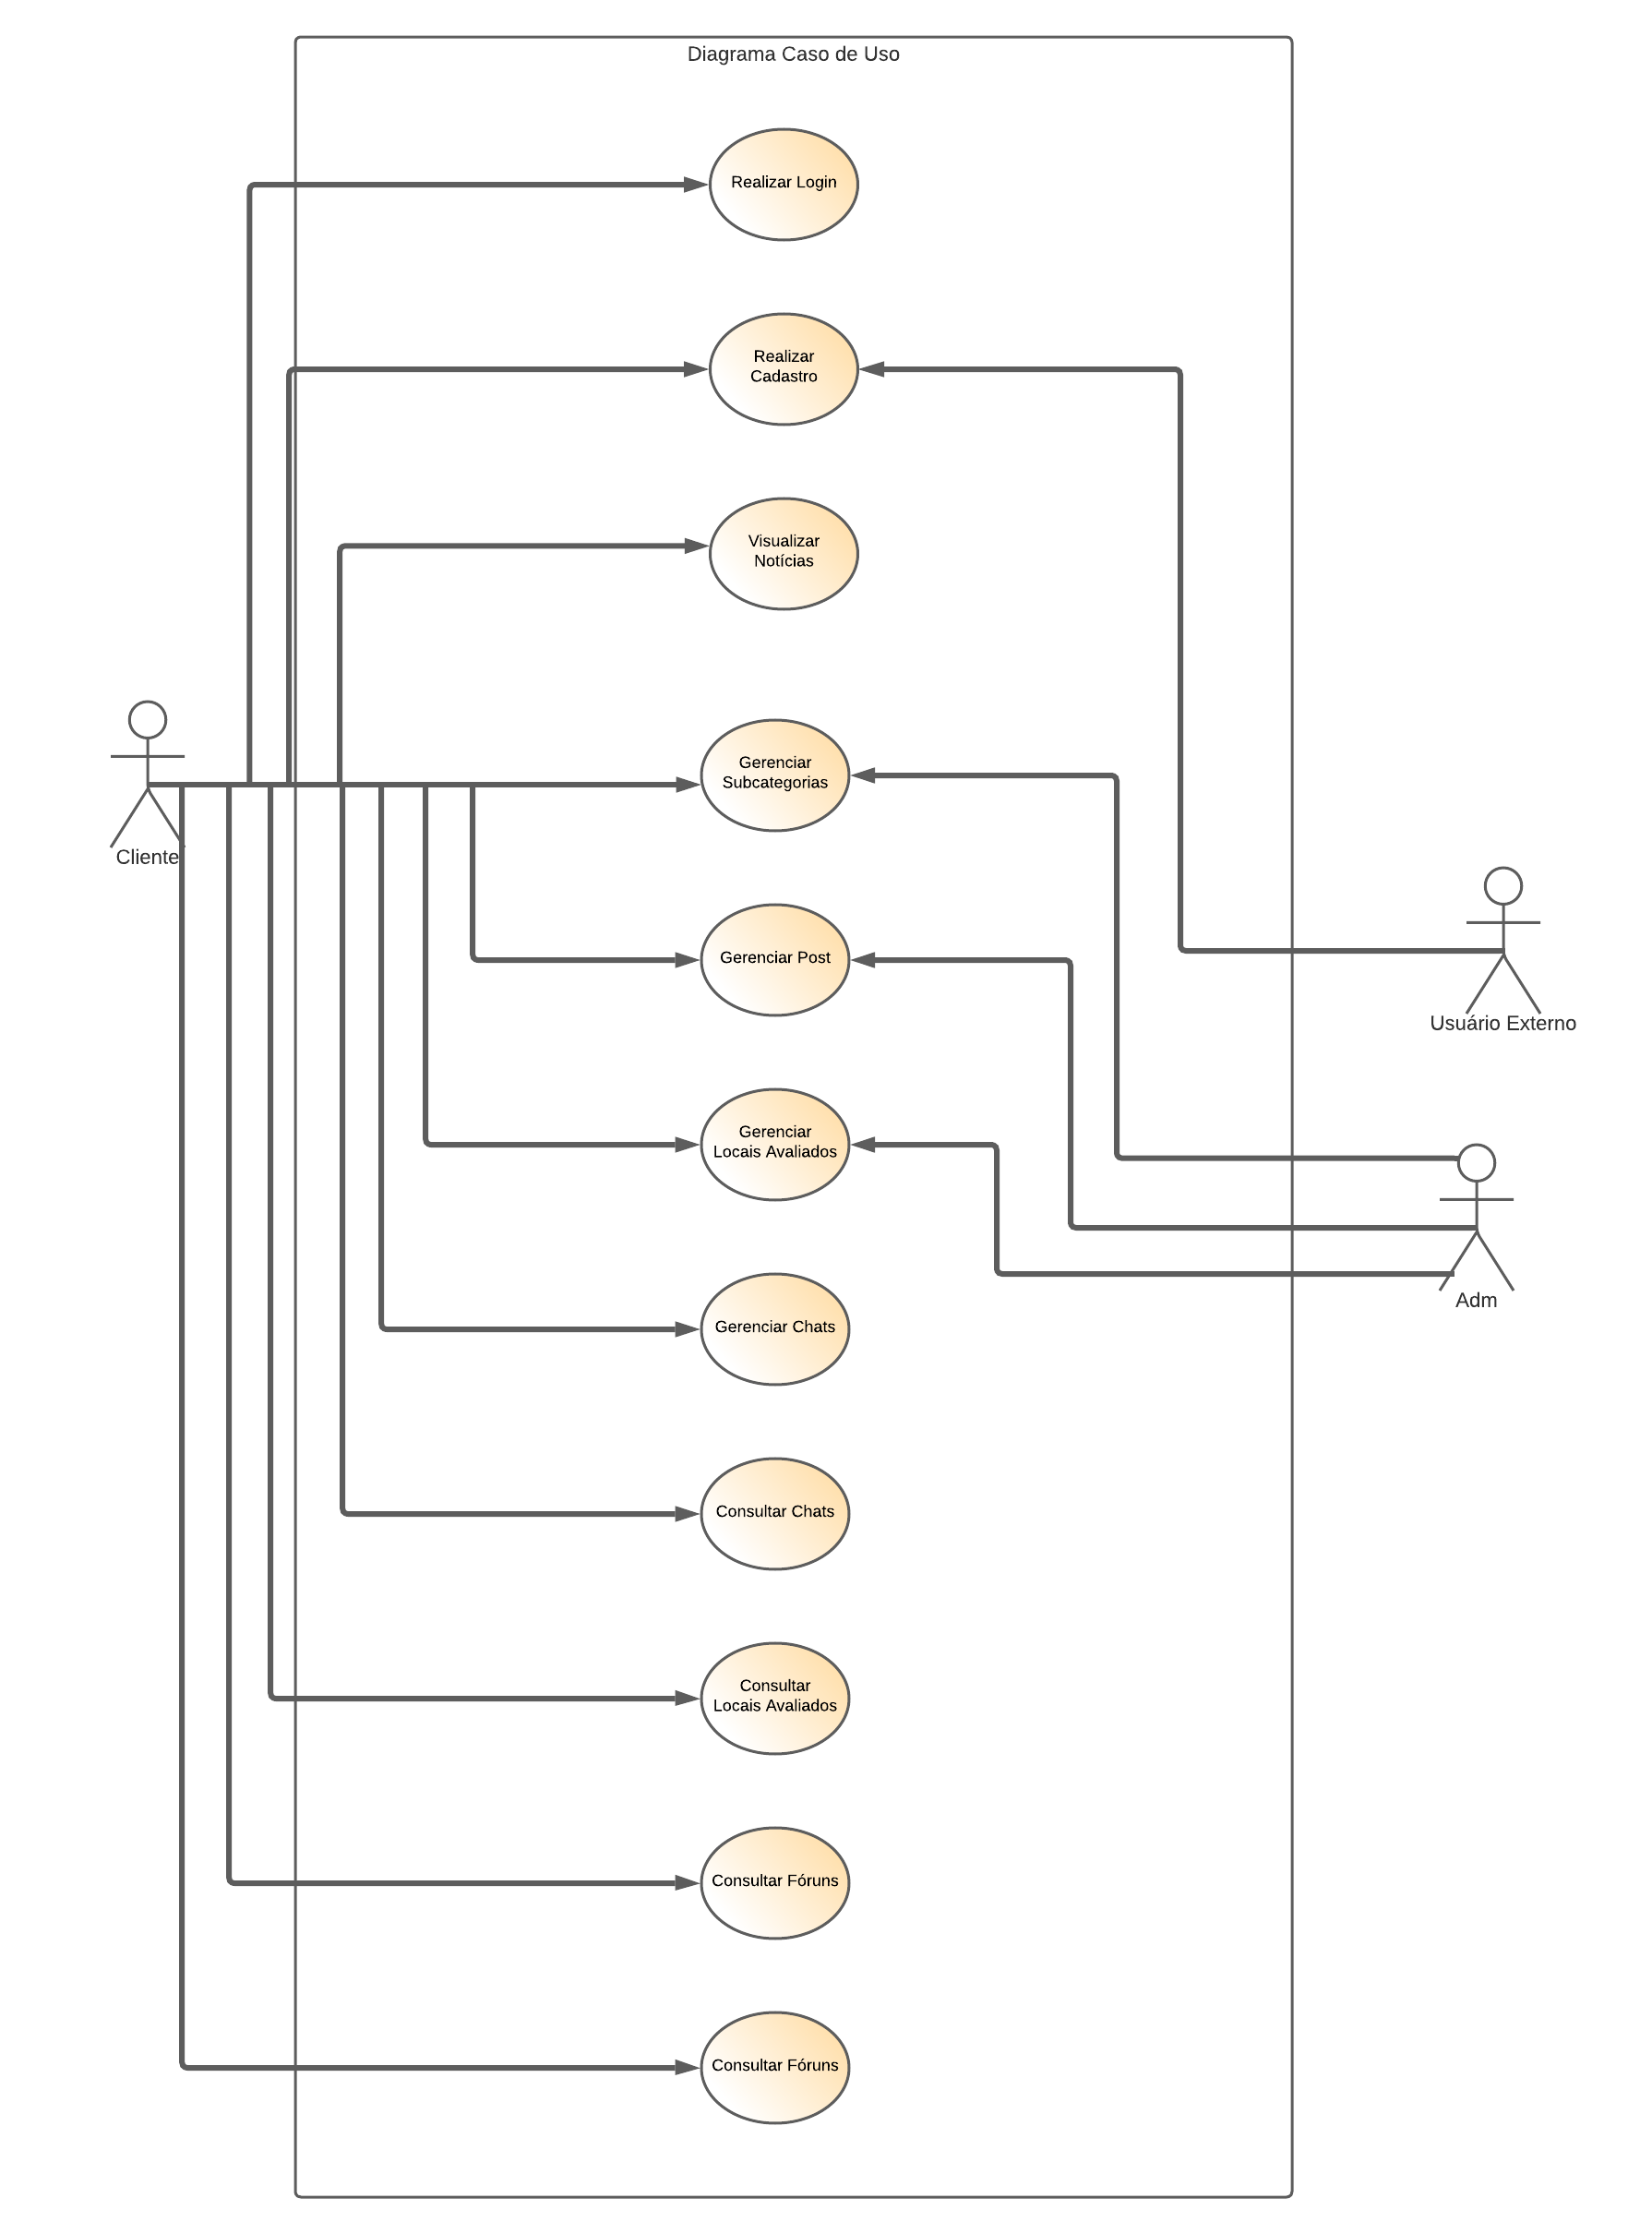
\includegraphics[width=0.90\textwidth]{anexos/Diagrama_em_branco.png}
	
	\legend{Fonte: Equipe diversaGente}
\end{figure}


%---------------------------------------------------------------------------------------
\section{Requisitos Funcionais, Não Funcionais e Regras de Negócios}

\explicacaoErro{Dentro desse capítulo também tem a regra de negócio e não citamos elas em nenhum momento. Adicionar um texto sobre ela para ser refereciada nesse capítulo}


A análise de requisitos do aplicativo está relacionada com as funcionalidades do sistema e com as prioridades diretamente ligadas a ele. Abaixo, eles estão divididos com suas respectivas funções que englobam tantos os requisitos funcionais, ou seja, declaração dos comportamentos que o sistema deve ter e os requisitos não funcionais que são as restrições colocadas sobre como o sistema deve realizar seus requisitos.

\explicacaoErro{Fazer o quadro sem longtable. APLICAR ISSO PARA TODAS AS OUTRAS TABELAS DENTRO DESSE CAPÍTULO.  }
\todo {Existem algumas correções para serem feitas dentro desses quadros.}

O  \autoref{tabela-requisitos-funcionais} mostra os requisitos funcionais  enquanto a \autoref{requisitos-nao-funcionais} mostra os requisitos não funcionais. 

\pagebreak

\begin{quadro}[htb]
	\centering
	\ABNTEXfontereduzida
	\caption[Requisitos Funcionais]{Requisitos Funcionais}
	\label{tabela-requisitos-funcionais}
\end{quadro}
\begin{longtable}{|p{2.0cm}|p{6.5cm}|p{6.5cm}|}
	\hline
	\thead{Código} & \thead{Requisito}  & \thead{Descrição} \\
	\hline
	RF01 &Visualizar notícias.  & Mostra as notícias dentro da aba news.
	Mostrar a imagem, título e início do texto que estão associados a notícia.
	Para cada notícia listada dentro da aba news, vai ser possível ter a opção de ir para um navegador externo ou continuar no app\\
	\hline
	RF02 & Gerenciar subcategorias. &
	O usuário consegue criar uma nova subcategoria dentro de uma categoria.
	O usuário que criou a subcategoria consegue editar o título das categorias criadas.
	O usuário consegue excluir a categoria que foi criada, recebendo um aviso se realmente é aquilo que ele deseja fazer.
	\\
	\hline
	RF03 & Gerenciar Post.   & O usuário consegue criar no novo post em dentro de uma subcategoria. 
	O usuário consegue editar um novo post dentro de uma subcategoria. 
	O usuário consegue excluir um post dentro de uma subcategoria\\
	\hline
	RF04 & Postar comentários dentro das subcategorias de discussões dos fóruns criados. & Ter um caixa de texto com um limite caracteres para o comentário ser postado
	Cada postagem precisa mostrar o usuário, data no formato DD/MM/AAAA.
	Mostrar toda a mensagem, sem a necessidade de clicar em ver mais.\\
	\hline
	RF05 & Compartilhar imagem dentro das postagens de subcategorias dos fóruns criados &
	Toda nova postagem vai ser necessário também ter um lugar para fazer o upload de uma imagem para ser postada.  \\
	\hline
	RF06 & Compartilhar nos aplicativos compatíveis as notícias e os posts das subcategorias de discussões dos fóruns criados.  & Apresentar uma lugar para que consiga compartilhar o post.
	Os posts precisam ser compartilhados com os aplicativos compatíveis.\\
	\hline
	RF07 & Favoritar mensagens dentro das subcategorias de discussões dos fóruns criados. & Deixar favoritar as mensagens. \\
	\hline
	RF08 & Gerenciar Locais Avaliados. & Fazer o cadastro de um local. Todas as informações cadastradas podem ser editadas. Permitir filtrar locais mais próximos do local que se encontra ou de um endereço desejado. \\
	\hline
	RF09 & Consultar Chats.   &Permitir que haja troca de mensagens instantâneas entre dois usuários.\\
	\hline
	RF10 &Receber notificações de mensagens novas. &
	Enviar uma notificação para o aparelho quando receber novas mensagens do chat, mostrando quem mandou a mensagem.  
	Mostrar quantas notificações possui  dentro do aplicativo.\\
	\hline
	RF11 & Filtrar conversas privadas do próprio usuário.  & Permitir pesquisar pelo nome do usuário dentro da aba conversar.\\
	\hline
	RF12 & Permitir que o usuário se cadastre na plataforma. & Conseguir criar um cadastro através de login social do google.\\
	\hline
	RF13 & Gerenciar Perfil.  &
	Permitir que o usuário altere os seus dados através de uma página de perfil.  \\
	\hline
	RF14 & Permitir que usuário bloqueie o recebimento de novas mensagens.  & Bloquear que usuários novos mandem mensagem. Bloquear que usuários que já houve troca de mensagem  envia novas mensagens.\\
	\hline
\end{longtable}
	\fonte{Equipe diversaGente (2022)}

\begin{quadro}[htb]
	\centering
	\ABNTEXfontereduzida
	\caption[Requisitos Não Funcionais]{Requisitos Não Funcionais}
	\label{requisitos-nao-funcionais}
	\begin{tabular}{|p{2.0cm}|p{6.5cm}|p{6.5cm}|}
		\hline
		\thead{Código} & \thead{Categoria}  & \thead{Requisito} \\
		\hline
		RNF01 & Compatibilidade &
		Deve ser compatível com o sistema operacional Android.\\
		\hline
		RNF02 & Disponibilidade & O sistema deve estar disponível 24 horas por dia, 7 dias por semana, com tolerância de 0,1\% de falhas. \\
		\hline
		RNF03 & Desempenho & O servidor deve responder em, no máximo, 0,4 segundos a todas as requisições recebidas. \\
		\hline
		RNF04 & Segurança & Para melhor análise e registro,os LOGS devem conter a data (dia, mês e ano), hora, minutos e uma breve descrição do registro.\\
		\hline
	\end{tabular}
	\fonte{Equipe diversaGente (2022)}
\end{quadro}

\begin{quadro}[htb]
	\centering
	\ABNTEXfontereduzida
	\caption[Regras de Negócio]{Regras de Negócio}
	\label{quadro-exemplo}
	\begin{tabular}{|p{3.3cm}|p{10.3cm}|}
		\hline
		\thead{Código} & \thead{Regra de negócio} \\
		\hline
		RN01 & É obrigatório que o usuário tenha uma conta Google para fazer o login na plataforma. \\
		\hline
		RN02 & Somente após finalizado o cadastro contendo todas as informações obrigatórias (login social, neuro interesse e motivação) o usuário obterá acesso à plataforma.\\
		\hline
		RN03 & Caso o usuário seja o criador de uma subcategoria, será possível editá-la e excluí-la.  \\
		\hline
		RN04 & Somente o usuário que é criador de uma avaliação da seção ‘Locais Avaliados’ é capaz de editá-la ou excluí-la. \\
		\hline
		RN05 & O recebimento de mensagens requer a permissão do usuário. \\
		\hline
		RN06 & Não devem haver subcategorias com o mesmo nome. \\
		\hline
		RN07 & Deverão ser mostradas de forma ranqueada as categorias, subcategorias e posts mais relevantes.\\
		\hline
		RN08 & É obrigatório que os posts publicados contenham título e texto.\\
		\hline
		RN09 & Caso o post seja editado, deve ser explicitado.\\
		\hline
	\end{tabular}
\fonte{Equipe diversaGente (2022)}
\end{quadro}\pagebreak

\section{Casos de Uso}
Os casos de uso a seguir representam uma possível utilização do nosso sistema por ator, seja ele o usuário ou administrador.\\

\begin{itemize}
	\item UC01: Fazer Login - Este uso de caso é abordado quando o cliente for fazer um cadastro na plataforma. O \autoref{casos-de-uso1} informa uma descrição, o fluxo básico de cadastro, um fluxo alternativo, pré-condições necessárias para conseguir fazer o uso de caso e pós-condições quando o uso de caso é concluído com sucesso.\\
	
	\explicacaoErro{Tirar a longtable. }
	
\end{itemize}

\begin{quadro}[htb]
	\centering
	\ABNTEXfontereduzida
	\caption[Caso de Uso Fazer Login]{Caso de Uso Fazer Login}
	\label{casos-de-uso1}
\end{quadro}
\begin{longtable}{|p{3.3cm}|p{12.3cm}|}
	\hline
	\thead{} & \thead{Ator} \\
	\hline
	Descrição & Ao realizar o processo de login, o usuário terá acesso a todas as funcionalidades do aplicativo como consultar o feed de notícias, ter acesso ao fórum podendo criar subcategorias e post e compartilhar informações nos canais de texto, enviar mensagens privadas a outras pessoas que também estão logadas no app e avaliar locais a partir da sua vivência deste estabelecimento \\
	\hline
	Fluxo Básico  & 
	\begin{enumerate}
		\item O usuário entra no aplicativo e visualiza a tela de login;
		\item O usuário insere seu email e senha;
		\item Usuário entra no aplicativo;
		\item O caso de uso é encerrado. 
	\end{enumerate}\\
	\hline
	Fluxo Alternativo  & O usuário esqueceu a senha:
	\begin{enumerate}
		\item O usuário entra no aplicativo e visualiza a tela de login;
		\item O usuário insere seu email e senha;
		\item O sistema informa que a senha inserida está incorreta.
		\item O usuário clica em "Esqueci minha senha";
		\item O sistema envia um e-mail para o ator para trocar a senha;
		\item O usuário abre o e-mail e redefine sua senha;
		\item O fluxo principal é recomeçado.
		\item O caso de uso é encerrado.
	\end{enumerate} \\
	\hline
	Fluxo Alternativo  &  Preenchimento incorreto da senha:
	\begin{enumerate}
		\item O usuário entra no aplicativo e visualiza a tela de login;
		\item O usuário insere seu email e senha;
		\item O sistema informa que a senha inserida está incorreta.
		\item O sistema informa que a senha inserida está incorreta.
		\item O caso de uso é encerrado. 
	\end{enumerate}\\
	\hline
	Fluxo Alternativo & Primeiro Acesso
	\begin{enumerate}
		\item O usuário entra no aplicativo e visualiza a tela de login;
		\item O usuário clica em "cadastrar";
		\item O sistema apresenta a tela de boas vindas;
		\item O usuário clica em "Avançar"
		\item O usuário insere as informações necessárias para o cadastramento no aplicativo;
		\item O usuário recebe a mensagem de "Cadastro feito com sucesso";
		\item O fluxo principal é começado para o usuário;
		\item O caso de uso é encerrado.
	\end{enumerate} \\
	\hline
	Fluxo Alternativo & Login Social (Google):
	\begin{enumerate}
		\item O usuário entra no aplicativo e visualiza a tela de login;
		\item O usuário clica no botão de realizar o login social;
		\item O sistema direciona o usuário para link do login social;
		\item O usuário faz sua autenticação com o email social e senha;
	\end{enumerate} \\ 
	\hline\pagebreak
	\hline
	&   
	\begin{enumerate}    
		\explicacaoErro{Quando se cria outra linha a numeração começa do 1.  }
		\item O usuário retorna para tela do aplicativo já sendo direcionado para o fluxo principal do app;
		\item O caso de uso é encerrado. 
	\end{enumerate} \\
	\hline
	Pré-condições & Ter acesso à internet, o aplicativo previamente instalado e uma conta Google.
	\hline
	Pós-condições & Acesso a homepage do aplicativo e de todas as funcionalidades existentes no sistema. \\
	\hline
\end{longtable}
\fonte{Equipe diversaGente (2022)}

%--------------------------------------------------------------

\begin{itemize}
	\item UC02: Efetuar Cadastro - Este uso de caso é abordado quando o cliente for fazer um cadastro na plataforma. O 	\autoref{casos-de-uso2} informa uma descrição, o fluxo básico de cadastro, um fluxo alternativo, pré-condições necessárias para conseguir fazer o uso de caso e pós-condições quando o uso de caso é concluído com sucesso. \\
\end{itemize}

	\explicacaoErro{Tirar a longtable }

\begin{quadro}[htb]
	\centering
	\ABNTEXfontereduzida
	\caption[Caso de Uso Efetuar Cadastro]{Caso de Uso Efetuar Cadastro}
	\label{casos-de-uso2}
\end{quadro}
\begin{longtable}{|p{3.3cm}|p{12.3cm}|}
	\hline
	\thead{} & \thead{Ator} \\
	\hline
	Descrição & Esse caso terá como funcionalidade o cadastrar novos usuários na aplicação.\\
	\hline
	Fluxo Básico  & 
	\begin{enumerate}
		\item O usuário entra no aplicativo e visualiza a tela de login;
		\item O usuário clica em "cadastrar";
		\item O sistema apresenta a tela de boas vindas;
		\item O usuário clica em "Avançar";
		\item O usuário clica em "Cadastrar no App";
		\item O usuário insere as informações necessárias para o cadastramento no aplicativo;
		\item É retornado ao usuário: "Cadastro realizado com sucesso";
	\end{enumerate}\\
	\hline	
	\hline
	&
	\begin{enumerate}
		\explicacaoErro{Quando se cria outra linha a numeração começa do 1.  }
		
		\item O fluxo principal é começado para o usuário;
		\item O caso de uso é encerrado.. 
	\end{enumerate}\\
	\hline
	Fluxo Alternativo  & Cadastro com a conta Google:
	\begin{enumerate}
		\item O usuário entra no aplicativo e visualiza a tela de login;
		\item O usuário clica em "cadastrar";
		\item O sistema apresenta a tela de boas vindas;
		\item O usuário clica em "Avançar";
		\item O usuário clica em "Cadastrar com o Google";
		\item O sistema irá direcioná-lo para sua conta google para permitir acesso;
		\item O usuário é retornado para o aplicativo e recebe a mensagem de "Cadastro feito com sucesso";
		\item  O fluxo principal é começado para o usuário;
		\item O caso de uso é encerrado.
	\end{enumerate}\\
	\hline
	Pré-condições & Ter acesso à internet e o aplicativo previamente instalado.\\
	\hline
	Pós-condições & O Visitante vai se tornar um novo usuário da aplicação.\\
	\hline
\end{longtable}
	\fonte{Equipe diversaGente (2022)}

%--------------------------------------------------------------

\begin{itemize}
	\item UC03: Editar perfil -  Este uso de caso é abordado quando o cliente for editar o seu perfil na plataforma.
	O \autoref{casos-de-uso3} informa uma descrição, o fluxo básico de cadastro, um fluxo alternativo, pré-
	condições necessárias para conseguir fazer o uso de caso e pós-condições quando o uso de
	caso é concluído com sucesso. \\

\end{itemize}

\explicacaoErro{Tirar a longtable}

\begin{quadro}[htb]
	\centering
	\ABNTEXfontereduzida
	\caption[Caso de Uso Editar Perfil]{Caso de Uso Editar Perfil}
	\label{casos-de-uso3}
\end{quadro}

%---------------------------------------------------------------

\begin{longtable}{|p{3.3cm}|p{12.3cm}|}
	\hline
	\thead{} & \thead{Ator} \\
	\hline
	Descrição & Esse caso de uso ocorre quando o usuário logado no aplicativo deseja alterar suas informações de perfil.\\
	\hline
	Fluxo Básico  &
	\begin{enumerate}
		\item O usuário seleciona a seção "Perfil";
		\item O usuário seleciona "Editar Perfil";
		\item O sistema exibe os dados do perfil: nome, data de nascimento, e-mail, neuro diversidades que tem interesse, abertura de mensagens privadas;
		\item O usuário seleciona o(s) dado(s) que deseja editar;
		\item O usuário atualiza as suas informações e pressiona no botão "Salvar";
		\item O sistema valida os dados conforme requeridos e atualiza o perfil do assinante;
		\item O caso de uso é encerrado. 
	\end{enumerate}\\
	\hline
	Pré-condições & Ter acesso à internet e estar previamente logado no aplicativo.\\
	\hline
	Pós-condições & Ao final das alterações feitas pelo usuário, a seção perfil deve estar atualizada.\\
	\hline
\end{longtable}
	\fonte{Equipe diversaGente (2022)}

%--------------------------------------------------------------

\begin{itemize}
	\item UC04: Consultar mensagens no Fórum - Este uso de caso é abordado quando o cliente for editar o seu perfil na plataforma.
	O \autoref{casos-de-uso3} informa uma descrição, o fluxo básico de cadastro, um fluxo alternativo, pré-
	condições necessárias para conseguir fazer o uso de caso e pós-condições quando o uso de
	caso é concluído com sucesso. \\

\end{itemize}

\explicacaoErro{Tirar a longtable para referencias a tabela corretamente. }

\begin{quadro}[htb]
	\centering
	\ABNTEXfontereduzida
	\label{quadro-exemplo}
	\caption[Caso de Uso Consultar mensagens do Fórum]{Caso de Uso Consultar mensagens do Fórum}
\end{quadro}
\begin{longtable}{|p{3.3cm}|p{12.3cm}|}
	\hline
	\thead{} & \thead{Ator} \\
	\hline
	Descrição & O cliente deve encontrar todas as mensagens ocorridas dentro das subcategorias.\\
	\hline
	Fluxo Básico  & 
	\begin{enumerate}
		\item O usuário seleciona a seção "Fórum";
		\item O usuário seleciona a categoria desejada;
	\end{enumerate}\\
	\hline
	
	\hline
	& 
	\begin{enumerate}
		\item O sistema mostra todas as subcategorias relacionadas categoria escolhida pelo usuário;
		\item O usuário escolhe uma subcategoria;
		\item O sistema mostra todas as mensagens ocorridas nesse canal de texto até o momento. 
		\item O caso de uso é encerrado.
	\end{enumerate}\\
	\hline
	Pré-condições & Ter acesso à internet e estar previamente logado no aplicativo.\\
	\hline
	Pós-condições & Ao final da escolha da subcategoria, deverá mostrar todas as mensagens do canal de texto.\\
	\hline
\end{longtable}
	\fonte{Equipe diversaGente (2022)}
%--------------------------------------------------------------

\begin{itemize}
	\item UC05: Remover mensagens no Fórum -Este uso de caso é abordado quando o cliente remover mensagens no fórum. O 	\autoref{casos-de-uso5} informa uma descrição, o fluxo básico de cadastro, pré-condições necessárias para conseguir fazer o uso de caso e pós-condições quando o uso de caso é concluído com sucesso. \\
\end{itemize}

\explicacaoErro{Tirar a longtable}

\begin{quadro}[htb]
	\centering
	\ABNTEXfontereduzida

%	\explicacaoErro{Informando no lugar errado. Quadro 11 remover mensagem do fórum }
	\caption[Caso de Uso Remover mensagens no Fórum]{Caso de Uso Remover mensagens no Fórum}
	\label{casos-de-uso5}
\end{quadro}
\begin{longtable}{|p{3.3cm}|p{12.3cm}|}
	\hline
	\thead{} & \thead{Ator} \\
	\hline
	Descrição & Ao criar uma subcategoria, o cliente poderá excluir sua própria mensagem dentro do canal de texto e poderá excluir as mensagens de outros dentro dessa subcategoria que ele criou. O Administrador terá permissão de excluir as mensagens das subcategorias, até mesmo do criador dela.\\
	\hline
	Fluxo Básico  & 
	Para o cliente:
	\begin{enumerate}
		\item O usuário seleciona a seção "Fórum";
		\item O usuário seleciona a categoria desejada;
		\item O sistema mostra todas as subcategorias relacionadas à categoria escolhida pelo usuário;
		\item O usuário escolhe uma subcategoria;
	\end{enumerate}
	\hline\pagebreak
	
	\hline
	& 
	\begin{enumerate}
		\item O sistema mostra todas as mensagens ocorridas nesse canal de texto até o momento. 
		\item O usuário seleciona a mensagem que deseja excluir;
		\item O sistema atualiza o canal de texto retirando a mensagem excluída. 
		\item O  caso de uso é encerrado. 
	\end{enumerate}\\
	\hline
	Fluxo Básico  & 
	Para o Administrador:
	\begin{enumerate}
		\item O administrador seleciona a seção "Fórum";
		\item O administrador seleciona a categoria desejada;
		\item O administrador mostra todas as subcategorias relacionadas à categoria escolhida pelo usuário;
		\item O administrador escolhe uma subcategoria;
		\item O sistema mostra todas as mensagens ocorridas nesse canal de texto até o momento. 
		\item O administrador seleciona a mensagem que deseja excluir;
		\item O sistema atualiza o canal de texto retirando a mensagem excluída. 
		\item O caso de uso é encerrado. 
	\end{enumerate}\\
	\hline
	Pré-condições & Para o Cliente: 
	
	O cliente deve estar logado no app e ser o criador do subcategoria escolhida.
	\hline
	Pré-Condições & Para o Administrador:
	
	Deve-ser ter o permissionamento de acesso necessário.
	\hline
	Pós-condições & O sistema deve atualizar o canal de texto já retirando a mensagem de texto excluída.
	\hline
\end{longtable}
	\fonte{Equipe diversaGente (2022)}
	
%--------------------------------------------------------------

\begin{itemize}
	\item UC06: Curtir mensagens no Fórum - Este uso de caso é abordado quando o cliente for curtir uma mensagem do fórum. O 	\autoref{casos-de-uso6} informa uma descrição, o fluxo básico de cadastro, pré-condições necessárias para conseguir fazer o uso de caso e pós-condições quando o uso de caso é concluído com sucesso.\\
\end{itemize}

\explicacaoErro{Tirar a longtable. }

\begin{quadro}[htb]
	\centering
	\ABNTEXfontereduzida
	\caption[Caso de Uso Curtir mensagens no Fórum]{Caso de Uso Curtir mensagens no Fórum}
	\label{casos-de-uso6}
\end{quadro}
\begin{longtable}{|p{3.3cm}|p{12.3cm}|}
	\hline
	\thead{} & \thead{Ator} \\
	\hline
	Descrição & O usuário poderá curtir uma mensagem de texto dentro das subcategorias.\\
	\hline
	Fluxo Básico  & 
	\begin{enumerate}
		\item O usuário seleciona a seção "Fórum";
		\item O usuário seleciona a categoria desejada;
		\item O sistema mostra todas as subcategorias relacionadas categoria escolhida pelo usuário;
		\item O usuário escolhe uma subcategoria;
		\item O sistema mostra todas as mensagens ocorridas nesse canal de texto até o momento. 
		\item  O usuário seleciona a mensagem desejada e clica em "curtir mensagem";
		\item  O sistema atualiza o canal de texto;
		\item  O caso de uso é encerrado;
	\end{enumerate}\\
	\hline
	Pré-condições & Ter acesso à internet e estar previamente logado no aplicativo.
	\hline
	Pós-condições & O sistema irá atualizar o número de curtidas da mensagem selecionada pelo usuário.\\
	\hline
\end{longtable}
	\fonte{Equipe diversaGente (2022)}
\pagebreak

%--------------------------------------------------------------

\begin{itemize}
	\item UC07: Criar categoria - Este uso de caso é abordado quando o cliente for curtir uma mensagem do fórum. O 	\autoref{casos-de-uso7}	informa uma descrição, o fluxo básico de cadastro, pré-condições necessárias para conseguir fazer o uso de caso e pós-condições quando o uso de caso é concluído com sucesso.\\
\end{itemize}

\explicacaoErro{Tirar a longtable.}

\begin{quadro}[htb]
	\centering
	\ABNTEXfontereduzida
	\caption[Caso de Uso Criar categoria]{Caso de Uso Criar categoria}
	\label{casos-de-uso7}
\end{quadro}
\begin{longtable}{|p{3.3cm}|p{12.3cm}|}
	\hline
	\thead{} & \thead{Ator} \\
	\hline
	Descrição & O Administrador tem permissão de criar uma categoria dentro do fórum.\\
	\hline
	Fluxo Básico  & 
	\begin{enumerate}
		\item O administrador seleciona a seção "Fórum";
		\item O administrador seleciona o botão "+";
		\item O sistema irá apresentar a opção "Criar uma Categoria";
		\item Ao clicar em criar uma categoria, o administrador deverá escrever o nome da categoria e clicar em "Criar canal de texto";
		\item O sistema atualizará com a nova categoria criada. 
		\item O caso de uso é encerrado. 
	\end{enumerate}\\
	\hline
	Pré-condições &O administrador deve ter a chave de permissão.
	\hline
	Pós-condições & O sistema mostrará a nova categoria criada pelo administrador e deve permitir que a partir dessa categoria sejam criadas subcategorias pelos usuários e administradores.\\
	\hline
\end{longtable}
	\fonte{Equipe diversaGente (2022)}
\pagebreak

%--------------------------------------------------------------

\begin{itemize}
	\item UC08: Criar uma subcategoria - Este uso de caso é abordado quando o cliente for criar uma subcategoria. O \autoref{casos-de-uso8}	informa uma descrição, o fluxo básico de cadastro, pré-condições necessárias para conseguir fazer o uso de caso e pós-condições quando o uso de caso é concluído com sucesso.\\
\end{itemize}

\explicacaoErro{Tirar a longtable.}

\begin{quadro}[htb]
	\centering
	\ABNTEXfontereduzida
	\caption[Caso de Uso Criar uma subcategoria]{Caso de Uso Criar uma subcategoria}
	\label{casos-de-uso8}
\end{quadro}
\begin{longtable}{|p{3.3cm}|p{12.3cm}|}
	\hline
	\thead{} & \thead{Ator} \\
	\hline
	Descrição & O cliente e/ou administrador devem conseguir criar subcategorias a partir das categorias já criadas pelo administrador.\\
	\hline
	Fluxo Básico  & 
	\begin{enumerate}
		\item O usuário seleciona a seção "Fórum";
		\item O usuário seleciona a categoria desejada;
		\item O usuário clica no botão "+" ao lado do nome da categoria selecionada;
		\item O usuário escreve o nome da subcategoria e clica em "Salvar"
		\item O sistema atualiza com a nova subcategoria criada. 
		\item O caso de uso é encerrado. 
	\end{enumerate}
	\hline
	Pré-condições & O cliente deve estar logado no app e o administrador deve ter a chave de permissão;
	\hline
	Pós-condições & O sistema mostrará a nova categoria criada pelo administrador ou usuário.\\
	\hline
\end{longtable}
	\fonte{Equipe diversaGente (2022)}
\pagebreak

%---------------------------------------------------------------

\begin{itemize}
	\item UC09: Remover uma subcategoria - Este uso de caso é abordado quando o cliente for remover uma subcategoria. O 	\autoref{casos-de-uso9}	informa uma descrição, o fluxo básico de cadastro, pré-condições necessárias para conseguir fazer o uso de caso e pós-condições quando o uso de caso é concluído com sucesso.\\
\end{itemize}

\explicacaoErro{Tirar a longtable.}

\begin{quadro}[htb]
	\centering
	\ABNTEXfontereduzida
	\caption[Caso de Uso Remover uma subcategoria]{Caso de Uso Remover uma subcategoria}
	\label{casos-de-uso9}
\end{quadro}

\begin{longtable}{|p{3.3cm}|p{12.3cm}|}
	\hline
	\thead{} & \thead{Ator} \\
	\hline
	Descrição & O cliente e/ou administrador devem conseguir remover uma subcategoria. \\
	\hline
	Fluxo Básico  & Para o cliente
	\begin{enumerate}
		\item O usuário seleciona a seção "Fórum";
		\item O usuário seleciona uma categoria;
		\item O sistema mostra todas as subcategoria existentes;
		\item O cliente seleciona a subcategoria desejada;
		\item O cliente pressiona a subcategoria;
		\item Caso o cliente seja o criador dessa subcategoria, o sistema irá mostrar uma pop-up perguntando para o usuário se ele deseja excluir a subcategoria criada. 
		\item O usuário clica em "Sim";
		\item O sistema exclui a subcategoria;
		\item O caso de uso é encerrado. 
	\end{enumerate}
	\hline
	Fluxo Básico  & Para o administrador
	\begin{enumerate}
		\item O administrador seleciona a seção "Fórum";
		\item O administrador seleciona uma categoria;
		\item O sistema mostra todas as subcategoria existentes;
	\end{enumerate}\\
	\hline
	&
	\begin{enumerate}
		\item O administrador seleciona a subcategoria desejada;
		\item O administrador pressiona a subcategoria;
		\item O sistema irá mostrar uma pop-up perguntando para o administrador se ele deseja excluir a subcategoria pressionada;
		\item O administrador clica em "Sim";
		\item O sistema exclui a subcategoria;
		\item O caso de uso é encerrado. 
	\end{enumerate}\\
	\hline
	Pré-condições & Para o cliente:
	
	O cliente deve estar logado no app e ser o criador do subcategoria escolhida. 
	\hline
	Pré-condições & Para o administrador:
	
	Deve-ser ter o permissionamento de acesso necessário.
	\hline
	Pós-condições & O sistema irá atualizar removendo a subcategoria selecionada.\\
	\hline
\end{longtable}
	\fonte{Equipe diversaGente (2022)}

%-----------------------------------------------------------

\begin{itemize}
	\item UC10: Criação do Local Avaliado - Este uso de caso é abordado quando o cliente for criar um local para ser avaliado. O \autoref{casos-de-uso10} informa uma descrição, o fluxo básico de cadastro, um fluxo de exceção, pré-condições necessárias para conseguir fazer o uso de caso e pós-condições quando o uso de caso é concluído com sucesso.\\	
\end{itemize}

\explicacaoErro{Tirar a longtable.}

\begin{quadro}[htb]
	\centering
	\ABNTEXfontereduzida
	\caption[Caso de Uso Criação do Local Avaliado]{Caso de Uso Criação do Local Avaliado}
	\label{casos-de-uso10}
\end{quadro}
\begin{longtable}{|p{3.3cm}|p{12.3cm}|}
	\hline
	\thead{} & \thead{Ator} \\
	\hline
	Descrição & O usuário poderá avaliar positivamente ou negativamente os estabelecimentos que ele queira recomendar para outras pessoas dentro da rede social.\\
	\hline
	Fluxo Básico  & 
	\begin{enumerate}
		\item O usuário clica na seção 'Locais Avaliados';
	\end{enumerate}
	\hline
	
	\hline
	&
	\begin{enumerate}
		\item O usuário clica na aba 'Meus Locais Avaliados';
		\item O usuário clica em "Adicionar Avaliação";
		\item O sistema fornece a parte de "Adicionar Avaliação";
		\item O usuário cadastra a avaliação e clica em "Salvar";
		\item O sistema busca identificar e confirmar os dados inseridos pelo usuário.
		\item O sistema retorna "Avaliação Adicionada" e adiciona na lista de locais avaliados;
		\item O caso de uso é encerrado.
	\end{enumerate}
	\hline
	Fluxo de Excessão & O usuário não insere todos os dados necessários: 
	\begin{enumerate}
		\item O usuário clica na aba 'Meus Locais Avaliados';
		\item O usuário clica em "Adicionar Avaliação";
		\item O sistema fornece a parte de "Adicionar Avaliação";
		\item O usuário cadastra a avaliação e clica em "Salvar";
		\item O sistema retorna os dados obrigatórios que o usuário não inseriu ao cadastrar e impede que a avaliação seja salva;
		\item O caso de uso é encerrado. 
	\end{enumerate}
	\hline
	Pré-condições & Ter acesso à internet e estar previamente logado no aplicativo.
	\hline
	Pós-condições & Apresentar o Local Avaliado cadastrado pelo usuário na aba ’Locais Avaliados’.
	\hline
\end{longtable}
	\fonte{Equipe diversaGente (2022)}
\pagebreak

%---------------------------------------------------------------

\begin{itemize}
	\item UC11: Consultar Locais Avaliados - Este uso de caso é abordado quando o cliente for consultar locais avaliados. O \autoref{casos-de-uso11} informa uma descrição, o fluxo básico de cadastro, pré-condições necessárias para conseguir fazer o uso de caso e pós-condições quando o uso de caso é concluído com sucesso.	
\end{itemize}

\explicacaoErro{Tirar a longtable}

\begin{quadro}[htb]
	\centering
	\ABNTEXfontereduzida
	\caption[Caso de Uso Consultar Locais Avaliados]{Consultar Locais Avaliados}
	\label{casos-de-uso11}
\end{quadro}
\begin{longtable}{|p{3.3cm}|p{12.3cm}|}
	\hline
	\thead{} & \thead{Ator} \\
	\hline
	Descrição & Consultar todos os locais avaliados já adicionados pelos usuários.\\
	\hline
	Fluxo Básico  & 
	\begin{enumerate}
		\item O usuário clica na seção 'Locais Avaliados';
		\item O usuário clica na aba 'Todos Locais Avaliados';  
		\item O usuário clica no nome de um local avaliado;
		\item O usuário visualiza a avaliação;
		\item O caso de uso é encerrado. 
	\end{enumerate}\\
	\hline
	Pré-condições & Ter acesso à internet e estar previamente logado no aplicativo.
	\hline
	Pós-condições & Apresentar todos os locais avaliados cadastrados e seus respectivos dados.\\
	\hline
\end{longtable}
	\fonte{Equipe diversaGente (2022)}

%---------------------------------------------------------------

\begin{itemize}
	\item UC12: Editar Locais Avaliados - Este uso de caso é abordado quando o cliente for editar um local avaliado. O 	\autoref{casos-de-uso12} informa uma descrição, o fluxo básico de cadastro, pré-condições necessárias para conseguir fazer o uso de caso e pós-condições quando o uso de caso é concluído com sucesso.\\
\end{itemize}

\explicacaoErro{Tirar a longtable}

\begin{quadro}[htb]
	\centering
	\ABNTEXfontereduzida
	\caption[Caso de Uso Editar Locais Avaliados]{Caso de Uso Editar Locais Avaliados}
	\label{casos-de-uso12}
\end{quadro}
\begin{longtable}{|p{3.3cm}|p{12.3cm}|}
	\hline
	\thead{} & \thead{Ator} \\
	\hline
	Descrição & O usuário poderá editar as informações inseridas por ele na aba de 'Meus Locais Avaliados'.\\
	\hline
	Fluxo Básico  &
	\begin{enumerate}
		\item O usuário clica na aba 'Meus Locais Avaliados';
		\item O usuário pressiona o local avaliado na qual ele quer editar;
		\item O sistema mostra uma pop-up com a opção "Editar Local Avaliado";
		\item O usuário clica em "Editar Local Avaliado";
		\item O usuário edita as informações e clica em "Salvar";
		\item O sistema confirmar os dados inseridos pelo usuário;
		\item O caso de uso é encerrado. 
	\end{enumerate}
	\hline
	Pré-condições & Ter acesso à internet, estar logado no aplicativo e ser o criador do local avaliado em questão.
	\hline
	Pós-condições & O sistema deve apresentar o local avaliado com as novas informações inseridas pelo usuário.
	\hline
\end{longtable}
	\fonte{Equipe diversaGente (2022)}
%---------------------------------------------------------------

\begin{itemize}
	\item UC13: Remover Local Avaliado - Este uso de caso é abordado quando o cliente remover um local avaliado. O \autoref{casos-de-uso13} informa uma descrição, o fluxo básico de cadastro, pré-condições necessárias para conseguir fazer o uso de caso e pós-condições quando o uso de caso é concluído com sucesso.\\		
\end{itemize}

\explicacaoErro{Tirar a longtable}

\begin{quadro}[htb]
	\centering
	\ABNTEXfontereduzida
	\caption[Caso de Uso Remover Local Avaliado]{Caso de Uso Remover Local Avaliado}
	\label{casos-de-uso13}
\end{quadro}
\begin{longtable}{|p{3.3cm}|p{12.3cm}|}
	\hline
	\thead{} & \thead{Ator} \\
	\hline
	Descrição &O usuário poderá excluir o local avaliado inserido por ele na aba de 'Meus Locais Avaliados'.\\
	\hline
	Fluxo Básico  & 
	\begin{enumerate}
		\item O usuário clica na seção 'Locais Avaliados';
		\item O usuário clica na aba 'Meus Locais Avaliados';
		\item O usuário pressiona o local avaliado na qual ele quer excluir;
	\end{enumerate}\\
	\hline
	
	\hline
	&
	\begin{enumerate}
		\item O sistema mostra uma pop-up com a opção "Excluir Local Avaliado"; 
		\item O usuário clica em "Excluir Local Avaliado";
		\item O usuário exclui local avaliado";
		\item O sistema atualiza e retorna com a mensagem "local excluído com sucesso";
		\item O caso de uso é encerrado. 
	\end{enumerate}\\
	\hline
	Pré-condições & Ter acesso à internet, estar previamente logado no aplicativo e ser o criador da avaliação de local em questão.
	\hline
	Pós-condições & O sistema deve excluir o local avaliado escolhido pelo usuário da lista "Meus Locais Avaliados" e "Locais Avalaidos".\\
	\hline
\end{longtable}
	\fonte{Equipe diversaGente (2022)}
	
%---------------------------------------------------------------

\begin{itemize}
	\item UC14: Visualizar Perfil dos usuários - Este uso de caso é abordado quando o cliente for visualizar um perfil de um outro usuário na plataforma. O \autoref{casos-de-uso14} informa uma descrição, o fluxo básico de cadastro, um fluxo alternativo, pré-condições necessárias para conseguir fazer o uso de caso e pós-condições quando o uso de caso é concluído com sucesso.\\	
\end{itemize}

\explicacaoErro{Tirar a longtable}

\begin{quadro}[htb]
	\centering
	\ABNTEXfontereduzida
	\caption[Caso de Uso Visualizar Perfil dos usuários]{Caso de Uso Visualizar Perfil dos usuários}
	\label{casos-de-uso14}
\end{quadro}
\begin{longtable}{|p{3.3cm}|p{12.3cm}|}
	\hline
	\thead{} & \thead{Ator} \\
	\hline
	Descrição & Visualiza perfil do cliente quando clica na foto de perfil ou no nome do usuário.\\
	\hline
	Fluxo Básico  & 
	\begin{enumerate}
		\item O usuário clica na imagem do usuário;
		\item O usuário visualiza o perfil de outro usuário;
		\item O caso de uso está encerrado.
	\end{enumerate}\\
	\hline
	Fluxo Alternativo & 
	\begin{enumerate}
		\item O usuário clica no nome do usuário;
		\item O usuário visualiza o perfil de outro usuário;
		\item O caso de uso está encerrado.
	\end{enumerate}\\
	\hline
	Pré-condições & Ter acesso à internet e estar logado previamente no aplicativo.\\
	\hline
	Pós-condições & O sistema irá mostrar uma nova tela com todas as informações do usuário escolhido.\\
	\hline
\end{longtable}
	\fonte{Equipe diversaGente (2022)}
\pagebreak

%---------------------------------------------------------------

\begin{itemize}
	\item UC15: Troca de mensagens de texto em chat individual - Este uso de caso é abordado quando o cliente for trocar uma mensagem de texto com outro perfil. O \autoref{casos-de-uso15} informa uma descrição, o fluxo básico de ação, um fluxo alternativo, pré-condições necessárias para conseguir fazer o uso de caso e pós-condições quando o uso de caso é concluído com sucesso.\\
\end{itemize}

\explicacaoErro{Tirar a longtable}

\begin{quadro}[htb]
	\centering
	\ABNTEXfontereduzida
	\caption[Caso de Uso Troca de mensagens de texto em chat individual]{Caso de Uso Troca de mensagens de texto em chat individual}
	\label{casos-de-uso15}
\end{quadro}

\begin{longtable}{|p{3.3cm}|p{12.3cm}|}
	\hline
	\thead{} & \thead{Ator} \\
	\hline
	Descrição &Nesse caso de uso, o usuário poderá enviar e receber mensagens por meio de um chat privado entre os usuários.\\
	\hline
	Fluxo Básico  & 
	\begin{enumerate}
		\item O usuário clica na aba "Chat";
		\item O usuário clica em um dos usuários que estão em sua lista;
		\item O usuário envia mensagem;
		\item O caso de uso é encerrado. 
	\end{enumerate}\\
	\hline
	Fluxo Alternativo & 
	Primeira vez do usuário enviando mensagem. 
	\begin{enumerate}
		\item O usuário clica na imagem ou no nome do outro usuário;
		\item O usuário visualiza o perfil desse usuário;
		\item O usuário clica em "Enviar Mensagem";
	\end{enumerate}\\
	\hline
	
	\hline
	&
	\begin{enumerate}
		\item O sistema abre o chat entre esses dois usuários;
		\item O usuário envia a mensagem;
		\item O caso de uso é encerrado 
	\end{enumerate}\\
	\hline
	Pré-condições & Ter acesso à internet e estar previamente logado no aplicativo\\
	\hline
	Pós-condições & O usuário deve ter sua mensagem entregue e recebida pelo outro usuário.\\
	\hline
\end{longtable}
	\fonte{Equipe diversaGente (2022)}

%---------------------------------------------------------------

\begin{itemize}
	\item UC16: Visualizar notícias -Este uso de caso é abordado quando o cliente quiser visualizar uma notícia dentro da plataforma. O \autoref{casos-de-uso16} informa uma descrição, o fluxo básico de ação, pré-condições necessárias para a realização do caso e pós-condições da ação.\\
\end{itemize}

\explicacaoErro{Tirar a longtable}

\begin{quadro}[htb]
	\centering
	\ABNTEXfontereduzida
	\caption[Caso de Uso Visualizar notícias]{Caso de Uso Visualizar notícias}
	\label{casos-de-uso16}
\end{quadro}
\begin{longtable}{|p{3.3cm}|p{12.3cm}|}
	\hline
	\thead{} & \thead{Ator} \\
	\hline
	Descrição & O usuário deverá visualizar todas as notícias dentro da seção "Feed de notícias".\\
	\hline
	Fluxo Básico  & 
	\begin{enumerate}
		\item O usuário logado entra na seção "Feed de notícias";
		\item O usuário visualiza as notícias;
		\item O caso de uso é encerrado. 
	\end{enumerate}\\
	\hline
	Fluxo Alternativo &
	\begin{enumerate}
		\item O usuário logado entra na seção "Feed de notícias";
		\item O usuário visualiza as notícias;
		\item O usuário clica em uma notícia;
		\item O sistema leva o usuário para uma nova tela com os detalhamentos da notícia clicada pelo usuário;
		\item O caso de uso é encerrado. 
	\end{enumerate}\\
	\hline
	Pré-condições & Ter acesso à internet e estar previamente logado no aplicativo.\\
	\hline
	Pós-condições & O sistema deve mostrar as notícias relacionadas ao tema de crianças neuro diversas.\\
	\hline
\end{longtable}
	\fonte{Equipe diversaGente (2022)}
	
%---------------------------------------------------------------

\begin{itemize}
	\item UC17: Criar um Post -Este uso de caso é abordado quando o cliente quiser criar uma postagem na plataforma. O 	\autoref{casos-de-uso17} informa uma descrição, o fluxo básico de ação, pré-condições necessárias para a realização do caso e pós-condições da ação.\\
\end{itemize}

\explicacaoErro{Tirar a longtable}

\begin{quadro}[htb]
	\centering
	\ABNTEXfontereduzida
	\caption[Caso de Uso Criar um Post]{Caso de Uso Criar um Post}
	\label{casos-de-uso17}
\end{quadro}
\begin{longtable}{|p{3.3cm}|p{12.3cm}|}
	\hline
	\thead{} & \thead{Ator} \\
	\hline
	Descrição & O usuário poderá criar um post a partir das subcategorias existentes. \\
	\hline
	Fluxo Básico  & 
	\begin{enumerate}
		\item O usuário seleciona uma subcategoria selecionada;
		\item O usuário clica no botão "+" ao lado do nome da subcategoria selecionada para criar o post;
		\item O usuário insere as informações necessárias para a criação do post;
		\item O usuário clica em "Criar Post"; 
		\item O caso de uso é encerrado. 
	\end{enumerate}\\
	\hline
	Pré-condições & Ter acesso à internet e estar previamente logado no aplicativo.\\
	\hline
	Pós-condições & O sistema deve permitir a criação do post feita pelo usuário.\\
	\hline
\end{longtable}
	\fonte{Equipe diversaGente (2022)}
%---------------------------------------------------------------

\begin{itemize}
	\item UC18: Remover um Post - Este uso de caso é abordado quando o cliente vai fazer a remoção de uma postagem previamente feita. O \autoref{casos-de-uso18} informa uma descrição, o fluxo básico de ação, um fluxo alternativo, pré-condições necessárias para a realização do caso e pós-condições da ação.\\
\end{itemize}

\explicacaoErro{Tirar a longtable}

\begin{quadro}[htb]
	\centering
	\ABNTEXfontereduzida
	\caption[Caso de Uso Remover um Post]{Caso de Uso Remover um Post}
	\label{casos-de-uso18}
\end{quadro}
\begin{longtable}{|p{3.3cm}|p{12.3cm}|}
	\hline
	\thead{} & \thead{Ator} \\
	\hline
	Descrição &O usuário poderá remover um post a partir das subcategorias existentes.\\
	\hline
	Fluxo Básico  & 
	\begin{enumerate}
		\item O usuário seleciona um post;
		\item O usuário clica na opção "Apagar Post";
		\item O sistema apaga o post criado pelo usuário;
		\item O caso de uso é encerrado.
	\end{enumerate}\\
	\hline
	Fluxo Alternativo & 
	O administrador remove um post
	\begin{enumerate}
		\item O administrador seleciona um post;
		\item O administrador clica na opção "Apagar Post";
		\item O sistema apaga o post criado pelo administrador;
		\item O caso de uso é encerrado. 
	\end{enumerate}\\
	\hline
	Pré-condições & Ter acesso à internet, estar previamente logado no aplicativo e já ter uma postagem própria criada.
	\hline
	Pós-condições & O sistema deve atualizar com o post excluído pelo usuário. \\
	\hline
\end{longtable}
	\fonte{Equipe diversaGente (2022)}

%---------------------------------------------------------------

\begin{itemize}
	\item UC19: Comentar Post - Este uso de caso é abordado quando o cliente fizer um comentário em uma postagem. O \autoref{casos-de-uso19} informa uma descrição, o fluxo básico de ação, pré-condições necessárias para a realização do caso e pós-condições da ação.\\
\end{itemize}

\explicacaoErro{Tirar a longtable}

\begin{quadro}[htb]
	\centering
	\ABNTEXfontereduzida
	\caption[Caso de Uso Comentar Post]{Caso de Uso Comentar Post}
	\label{casos-de-uso19}
\end{quadro}
\begin{longtable}{|p{3.3cm}|p{12.3cm}|}
	\hline
	\thead{} & \thead{Ator} \\
	\hline
	Descrição & O usuário poderá comentar um post a partir das subcategorias existentes. \\
	\hline
	Fluxo Básico  & 
	\begin{enumerate}
		\item O usuário seleciona um post;
		\item O usuário clica na opção "Comentar";
		\item O usuário adiciona um comentário no post seleciona;
		\item O caso de uso é encerrado. 
	\end{enumerate}
	\hline
	Pré-condições & Ter acesso à internet e estar previamente logado no aplicativo
	\hline
	Pós-condições & O sistema deve mostrar o comentário do usuário no post selecionado.
	\hline
\end{longtable}
	\fonte{Equipe diversaGente (2022)}

%---------------------------------------------------------------

\begin{itemize}
	\item UC20: Curtir Post - Este uso de caso é abordado quando o cliente realiza a ação de curtir uma postagem. O \autoref{casos-de-uso20} informa uma descrição, o fluxo básico de ação, pré-condições necessárias e pós-condições da ação.\\
	
		
\end{itemize}

\explicacaoErro{Tirar a longtable}

\begin{quadro}[htb]
	\centering
	\ABNTEXfontereduzida
	\caption[Caso de Uso Curtir Post]{Caso de Uso Curtir Post}
	\label{casos-de-uso20}
\end{quadro}
\begin{longtable}{|p{3.3cm}|p{12.3cm}|}
	\hline
	\thead{} & \thead{Ator} \\
	\hline
	Descrição & O usuário poderá curtir um post criado na subcategoria.\\
	\hline
	Fluxo Básico  & 
	\begin{enumerate}
		\item O usuário seleciona um post;
		\item O usuário clica em "Curtir";
		\item O caso de uso é encerrado.
	\end{enumerate}\\
	\hline
	Pré-condições & Ter acesso à internet e estar previamente logado no aplicativo
	\hline
	Pós-condições & O sistema deve atualizar as curtidas realizadas no post do usuário.\\
	\hline
\end{longtable}
	\fonte{Equipe diversaGente (2022)}
\pagebreak

%---------------------------------------------------------------

\begin{itemize}
	\item UC21: Comentar notícias - Este uso de caso é abordado quando o cliente vai fazer um comentário em uma notícia. O \autoref{casos-de-uso21} informa uma descrição, o fluxo básico do comentário, pré-condições necessárias para ser possível comentar e as condições pós o comentário ser realizado.\\
\end{itemize}

\explicacaoErro{Tirar a longtable}

\begin{quadro}[htb]
	\centering
	\ABNTEXfontereduzida
	\caption[Caso de Uso Comentar notícias]{Caso de Uso Comentar notícias}
	\label{casos-de-uso21}
\end{quadro}
\begin{longtable}{|p{3.3cm}|p{12.3cm}|}
	\hline
	\thead{} & \thead{Ator} \\
	\hline
	Descrição & O usuário deve conseguir comentar uma notícias na seção "Feed de notícias". \\
	\hline
	Fluxo Básico  & 
	\begin{enumerate}
		\item O usuário logado entra na seção "Feed de notícias";
		\item O usuário visualiza as notícias;
		\item O usuário clica em uma notícia;
		\item O sistema leva o usuário para uma nova tela com os detalhamentos da notícia clicada pelo usuário;
		\item O usuário escreve seu comentário;
		\item O usuário clica em "Comentar";
		\item O caso de uso é encerrado. 
	\end{enumerate}
	\hline
	Pré-condições & Ter acesso à internet e estar previamente logado no aplicativo
	\hline
	Pós-condições & Após o usuário salvar seu comentário, o sistema deve apresentar o comentário realizado pelo usuário; 
	\hline
\end{longtable}
	\fonte{Equipe diversaGente (2022)}

\subsection{Entregas}

Durante a disciplina a equipe teve algumas entregas a serem feitas, para o projeto ser aprovado pelos Professores responsáveis e também acompanhar o desenvolvimento e dar sugestões caso necessário. 

Foi exigido que para a aplicação escolhida precisaria ter ao menos um processo, além de todos os CRUDS necessários para o funcionamento correto da aplicação. 

Foram planejadas quatro entregas, a primeira para mostrar as tecnologias usadas na aplicação e mostrar um desenho da arquitetura de como as camadas e ferramentas serão integradas. A segunda entrega para mostrar a POC, mostrar o ambiente de produção funcionando e as integrações necessárias para testar a arquitetura proposta pela equipe Garage Launcher. Na terceira, a entrega do MVP, é necessário entregar a aplicação funcionando em ambiente de produção com ao menos um processo implementado e finalmente na quarta entrega, a final, com todos os CRUDs e processos prontos para apresentação para a banca de Professores. A tabela abaixo mostra as três principais fases de entrega e suas respectivas funcionalidades.


% Please add the following required packages to your document preamble:
% \usepackage{lscape}
% \usepackage{longtable}
% Note: It may be necessary to compile the document several times to get a multi-page table to line up properly
\renewcommand\LTcaptype{quadro}
\begin{landscape}
	\begin{longtable}[]{|l|c|c|c|}
		
		\caption[Caso de Uso Comentar notícias]{Caso de Uso Comentar notícias}
		\hline
		& Prova Conceito  &  MVP  & Projeto Finalizado   \\ \hline
		\endfirsthead
		%
		\multicolumn{4}{c}{\scriptsize Fonte: Autor.}%
		{{\bfseries Table \thetable\ continued from previous page}} \\
		\hline
		& & &  \\ \hline
		\endhead
		%
		Ambientalização & X & X & X \\ \hline
		Integração de ferramentas & X & X & X \\ \hline
		Fórum &  & X & X \\ \hline
		Chat  &  &  & X \\ \hline
		Avaliações &  & X & X \\ \hline
		Feed de notícias &  &  & X \\ \hline
		
		\caption*{Fonte: Equipe diversaGente}
	\end{longtable}
\end{landscape}

\subsection{Escolhas e Descartes}

De início tínhamos acertado que iríamos usar o Firebase para fazer a autenticação da nossa aplicação, entretanto resolvemos usar o OAuth2 que nada mais é que um protocolo de autorização que permite que uma aplicação se autentique em outra. Essa mudança foi devido aos conhecimentos da equipe para aplicar o protocolo que estava mais próximo daquilo que a equipe tinha que entregar, além de ser uma aplicação mais simples, leve e rápida para implementar e autenticar os nossos usuários dentro do nosso aplicativo. 

\section{Critérios de segurança}


A aplicação está de acordo com a Lei Geral de Proteção de Dados (LGPD, Lei nº13.709/2018). Os dados que serão coletados e utilizados são: Como o usuário gostaria de ser chamado, foto do usuário opcional, data de nascimento, e-mail, neuroatipicidade da criança, localização aproximada opcional e senha. Não é obrigatório a publicação nem carregamento de dados pessoais que não queira disponibilizar ao público. 

Para maior garantia de segurança, o armazenamento da senha será feito pela própria Google, com o uso da autenticação OAuth2.0 e os dados dos usuários obterão total sigilo, já que estarão assegurados pelo protocolo de autenticação da conta Google, sendo visíveis apenas pelo próprio usuário e por administradores do sistema em situações que sejam necessárias. 

Os dados não sensíveis dos usuários (como nome de usuário e foto de perfil) serão visíveis para todos os usuários cadastrados, já dados sensíveis serão visualizáveis apenas pelo próprio usuário e, se necessário, pelos administradores da plataforma. Os dados armazenados terão a sua integridade mantida, ou seja, não sofrerão alterações indevidas sem autorização do usuário, para que não possam vir a corromper a veracidade das informações. 

Caso o usuário opte por encerrar sua conta, os seus dados pessoais não ficarão mais visíveis para outros usuários e seu perfil não deverá mais ser encontrado nas buscas dentro do aplicativo. Em 30 dias após o encerramento da conta todos os dados e informações da conta encerrada serão excluídos. 


\section{Viabilidade Financeira}
% ---
\subsection{Custos}
% ---
Nesta seção serão considerados os custos das ferramentas pagas cujo o uso já está previsto no projeto da aplicação. 

Como ferramentas pagas imprescindíveis para o funcionamento da infraestrutura da aplicação prevê-se:

\begin{quadro}[htb]
	\centering
	\ABNTEXfontereduzida
	\caption[Custo das ferramentas]{Custo das ferramentas}
	\label{quadro-exemplo}
	\begin{tabular}{|p{4.0cm}|p{4.0cm}|p{3.0cm}|}
		\hline
		\thead{Ferramenta} & \thead{Uso}  & \thead{Custo mensal\\(em dólares)} \\
		\hline
		Heroku & API e Banco de dados  & 25,00  \\
		\hline
		Cloudinary & Servidor de arquivos &
		89,00 \\
		\hline
	\end{tabular}
\end{quadro}

Para o recurso de envio e recebimento de e-mails estão sendo estudadas duas ferramentas: 

\begin{quadro}[htb]
	\centering
	\ABNTEXfontereduzida
	\caption[Custo das ferramentas de email]{Custo das ferramentas de email}
	\label{quadro-exemplo}
	\begin{tabular}{|p{4.0cm}|p{4.0cm}|p{3.0cm}|}
		\hline
		\thead{Ferramenta} & \thead{Uso}  & \thead{Custo mensal\\(em dólares)} \\
		\hline
		Simple Email Service & Envio e recebimento de e-mails & 0,10*\\
		\hline
	\end{tabular}
\end{quadro}

*O custo de U\$0,10 diz respeito a um volume de até mil e-mails enviados/recebidos pela ferramenta e, considerando o alcance inicial da aplicação, pode-se afirmar que este seria o gasto mensal referente ao recurso durante um considerável período de tempo, e por se tratar de um melhor custo benefício, provavelmente será a ferramenta escolhida. 

Tendo em vista que o aplicativo também terá sua versão mobile, devem ser considerados os custos para a publicação nas lojas virtuais mobile: 

\begin{quadro}[htb]
	\centering
	\ABNTEXfontereduzida
	\caption[Custo da ferramenta de disponibilização]{Custo da ferramenta de disponibilização}
	\label{quadro-exemplo}
	\begin{tabular}{|p{4.0cm}|p{4.0cm}|p{3.0cm}|}
		\hline
		\thead{Store de\\ disponibilização} & \thead{Custo\\(em dólares)} \\
		\hline
		Play Store & 25,00 \\
		\hline
	\end{tabular}
\end{quadro}

Dessa forma, pode-se considerar como custo inicial, inserindo a postagem, o valor de U\$139,10 e após a postagem, o custo de mantenimento mensal passa a ser U\$114,10.

\subsection{Receitas}

Neste tópico será abordada a metodologia de captação de receitas que será utilizada na aplicação.

O instrumento escolhido como gerador de capital para o diversaGente é a Google AdSense, uma ferramenta de anúncios gratuita da Google. A escolha dessa ferramenta foi baseada, principalmente, no critério de confiabilidade, já que se trata de um produto imensamente utilizado nos dias atuais. Além de ser uma ferramenta muito disseminada, ela tem uma estrutura de implantação muito simples - basta inserir o código de anúncio no seu site ou aplicação e definir os espaços onde serão exibidos -, dessa forma pode-se obter maior agilidade na capitalização.

A Google AdSense tem duas maneiras de capitalizar. A primeira delas é com base nas impressões dos usuários geradas nos anúncios expostos e, a segunda, é com base nos cliques dos usuários nos anúncios; para ambas as maneirasa porcentagem de receita é a mesma, 68\%. Para melhor elucidar sobre este ganho, a própria Google expõe o seguinte exemplo: "Acreditamos que nossa divisão da rec seja extremamente competitiva. No entanto, as divisões de receita analisadas de modo isolado podem ser ilusórias. Desse modo, recomendamos que você se concentre na receita total gerada para seu site. Por exemplo, se o leilão do Google de um inventário de anúncios no seu site gerar R\$ 100,00, com a divisão da receita de 68\%, você receberia R\$ 68,00 por meio do Google AdSense.(...)". 

A Google também garante que, devido ao alto nível de competitividade da empresa e de sua ferramenta de anúncios, aqueles que utilizarem a Google AdSense estarão ganhando o máximo que o mercado possibilita

O exemplo exposto e esta garantia podem ser conferidos no link:\\ \hyperlink{Link da Google AdSense}{https://support.google.com/adsense/answer/6242051?hl=pt-BR#zippy=}

